\documentclass[1p]{elsarticle_modified}
%\bibliographystyle{elsarticle-num}

%\usepackage[colorlinks]{hyperref}
%\usepackage{abbrmath_seonhwa} %\Abb, \Ascr, \Acal ,\Abf, \Afrak
\usepackage{amsfonts}
\usepackage{amssymb}
\usepackage{amsmath}
\usepackage{amsthm}
\usepackage{scalefnt}
\usepackage{amsbsy}
\usepackage{kotex}
\usepackage{caption}
\usepackage{subfig}
\usepackage{color}
\usepackage{graphicx}
\usepackage{xcolor} %% white, black, red, green, blue, cyan, magenta, yellow
\usepackage{float}
\usepackage{setspace}
\usepackage{hyperref}

\usepackage{tikz}
\usetikzlibrary{arrows}

\usepackage{multirow}
\usepackage{array} % fixed length table
\usepackage{hhline}

%%%%%%%%%%%%%%%%%%%%%
\makeatletter
\renewcommand*\env@matrix[1][\arraystretch]{%
	\edef\arraystretch{#1}%
	\hskip -\arraycolsep
	\let\@ifnextchar\new@ifnextchar
	\array{*\c@MaxMatrixCols c}}
\makeatother %https://tex.stackexchange.com/questions/14071/how-can-i-increase-the-line-spacing-in-a-matrix
%%%%%%%%%%%%%%%

\usepackage[normalem]{ulem}

\newcommand{\msout}[1]{\ifmmode\text{\sout{\ensuremath{#1}}}\else\sout{#1}\fi}
%SOURCE: \msout is \stkout macro in https://tex.stackexchange.com/questions/20609/strikeout-in-math-mode

\newcommand{\cancel}[1]{
	\ifmmode
	{\color{red}\msout{#1}}
	\else
	{\color{red}\sout{#1}}
	\fi
}

\newcommand{\add}[1]{
	{\color{blue}\uwave{#1}}
}

\newcommand{\replace}[2]{
	\ifmmode
	{\color{red}\msout{#1}}{\color{blue}\uwave{#2}}
	\else
	{\color{red}\sout{#1}}{\color{blue}\uwave{#2}}
	\fi
}

\newcommand{\Sol}{\mathcal{S}} %segment
\newcommand{\D}{D} %diagram
\newcommand{\A}{\mathcal{A}} %arc


%%%%%%%%%%%%%%%%%%%%%%%%%%%%%5 test

\def\sl{\operatorname{\textup{SL}}(2,\Cbb)}
\def\psl{\operatorname{\textup{PSL}}(2,\Cbb)}
\def\quan{\mkern 1mu \triangleright \mkern 1mu}

\theoremstyle{definition}
\newtheorem{thm}{Theorem}[section]
\newtheorem{prop}[thm]{Proposition}
\newtheorem{lem}[thm]{Lemma}
\newtheorem{ques}[thm]{Question}
\newtheorem{cor}[thm]{Corollary}
\newtheorem{defn}[thm]{Definition}
\newtheorem{exam}[thm]{Example}
\newtheorem{rmk}[thm]{Remark}
\newtheorem{alg}[thm]{Algorithm}

\newcommand{\I}{\sqrt{-1}}
\begin{document}

%\begin{frontmatter}
%
%\title{Boundary parabolic representations of knots up to 8 crossings}
%
%%% Group authors per affiliation:
%\author{Yunhi Cho} 
%\address{Department of Mathematics, University of Seoul, Seoul, Korea}
%\ead{yhcho@uos.ac.kr}
%
%
%\author{Seonhwa Kim} %\fnref{s_kim}}
%\address{Center for Geometry and Physics, Institute for Basic Science, Pohang, 37673, Korea}
%\ead{ryeona17@ibs.re.kr}
%
%\author{Hyuk Kim}
%\address{Department of Mathematical Sciences, Seoul National University, Seoul 08826, Korea}
%\ead{hyukkim@snu.ac.kr}
%
%\author{Seokbeom Yoon}
%\address{Department of Mathematical Sciences, Seoul National University, Seoul, 08826,  Korea}
%\ead{sbyoon15@snu.ac.kr}
%
%\begin{abstract}
%We find all boundary parabolic representation of knots up to 8 crossings.
%
%\end{abstract}
%\begin{keyword}
%    \MSC[2010] 57M25 
%\end{keyword}
%
%\end{frontmatter}

%\linenumbers
%\tableofcontents
%
\newcommand\colored[1]{\textcolor{white}{\rule[-0.35ex]{0.8em}{1.4ex}}\kern-0.8em\color{red} #1}%
%\newcommand\colored[1]{\textcolor{white}{ #1}\kern-2.17ex	\textcolor{white}{ #1}\kern-1.81ex	\textcolor{white}{ #1}\kern-2.15ex\color{red}#1	}

{\Large $\underline{12a_{0505}~(K12a_{0505})}$}

\setlength{\tabcolsep}{10pt}
\renewcommand{\arraystretch}{1.6}
\vspace{1cm}\begin{tabular}{m{100pt}>{\centering\arraybackslash}m{274pt}}
\multirow{5}{120pt}{
	\centering
	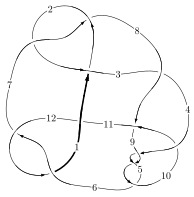
\includegraphics[width=112pt]{../../../GIT/diagram.site/Diagrams/png/1306_12a_0505.png}\\
\ \ \ A knot diagram\footnotemark}&
\allowdisplaybreaks
\textbf{Linearized knot diagam} \\
\cline{2-2}
 &
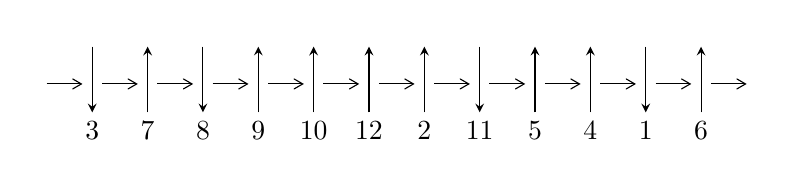
\begin{tikzpicture}[x=20pt, y=17pt]
	% nodes
	\node (C0) at (0, 0) {};
	\node (C1) at (1, 0) {};
	\node (C1U) at (1, +1) {};
	\node (C1D) at (1, -1) {3};

	\node (C2) at (2, 0) {};
	\node (C2U) at (2, +1) {};
	\node (C2D) at (2, -1) {7};

	\node (C3) at (3, 0) {};
	\node (C3U) at (3, +1) {};
	\node (C3D) at (3, -1) {8};

	\node (C4) at (4, 0) {};
	\node (C4U) at (4, +1) {};
	\node (C4D) at (4, -1) {9};

	\node (C5) at (5, 0) {};
	\node (C5U) at (5, +1) {};
	\node (C5D) at (5, -1) {10};

	\node (C6) at (6, 0) {};
	\node (C6U) at (6, +1) {};
	\node (C6D) at (6, -1) {12};

	\node (C7) at (7, 0) {};
	\node (C7U) at (7, +1) {};
	\node (C7D) at (7, -1) {2};

	\node (C8) at (8, 0) {};
	\node (C8U) at (8, +1) {};
	\node (C8D) at (8, -1) {11};

	\node (C9) at (9, 0) {};
	\node (C9U) at (9, +1) {};
	\node (C9D) at (9, -1) {5};

	\node (C10) at (10, 0) {};
	\node (C10U) at (10, +1) {};
	\node (C10D) at (10, -1) {4};

	\node (C11) at (11, 0) {};
	\node (C11U) at (11, +1) {};
	\node (C11D) at (11, -1) {1};

	\node (C12) at (12, 0) {};
	\node (C12U) at (12, +1) {};
	\node (C12D) at (12, -1) {6};
	\node (C13) at (13, 0) {};

	% arrows
	\draw[->,>={angle 60}]
	(C0) edge (C1) (C1) edge (C2) (C2) edge (C3) (C3) edge (C4) (C4) edge (C5) (C5) edge (C6) (C6) edge (C7) (C7) edge (C8) (C8) edge (C9) (C9) edge (C10) (C10) edge (C11) (C11) edge (C12) (C12) edge (C13) ;	\draw[->,>=stealth]
	(C1U) edge (C1D) (C2D) edge (C2U) (C3U) edge (C3D) (C4D) edge (C4U) (C5D) edge (C5U) (C6D) edge (C6U) (C7D) edge (C7U) (C8U) edge (C8D) (C9D) edge (C9U) (C10D) edge (C10U) (C11U) edge (C11D) (C12D) edge (C12U) ;
	\end{tikzpicture} \\
\hhline{~~} \\& 
\textbf{Solving Sequence} \\ \cline{2-2} 
 &
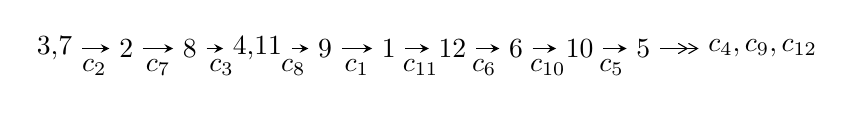
\begin{tikzpicture}[x=23pt, y=7pt]
	% node
	\node (A0) at (-1/8, 0) {3,7};
	\node (A1) at (1, 0) {2};
	\node (A2) at (2, 0) {8};
	\node (A3) at (49/16, 0) {4,11};
	\node (A4) at (33/8, 0) {9};
	\node (A5) at (41/8, 0) {1};
	\node (A6) at (49/8, 0) {12};
	\node (A7) at (57/8, 0) {6};
	\node (A8) at (65/8, 0) {10};
	\node (A9) at (73/8, 0) {5};
	\node (C1) at (1/2, -1) {$c_{2}$};
	\node (C2) at (3/2, -1) {$c_{7}$};
	\node (C3) at (5/2, -1) {$c_{3}$};
	\node (C4) at (29/8, -1) {$c_{8}$};
	\node (C5) at (37/8, -1) {$c_{1}$};
	\node (C6) at (45/8, -1) {$c_{11}$};
	\node (C7) at (53/8, -1) {$c_{6}$};
	\node (C8) at (61/8, -1) {$c_{10}$};
	\node (C9) at (69/8, -1) {$c_{5}$};
	\node (A10) at (11, 0) {$c_{4},c_{9},c_{12}$};

	% edge
	\draw[->,>=stealth]	
	(A0) edge (A1) (A1) edge (A2) (A2) edge (A3) (A3) edge (A4) (A4) edge (A5) (A5) edge (A6) (A6) edge (A7) (A7) edge (A8) (A8) edge (A9) ;
	\draw[->>,>={angle 60}]	
	(A9) edge (A10);
\end{tikzpicture} \\ 

\end{tabular} \\

\footnotetext{
The image of knot diagram is generated by the software ``\textbf{Draw programme}" developed by Andrew Bartholomew(\url{http://www.layer8.co.uk/maths/draw/index.htm\#Running-draw}), where we modified some parts for our purpose(\url{https://github.com/CATsTAILs/LinksPainter}).
}\phantom \\ \newline 
\centering \textbf{Ideals for irreducible components\footnotemark of $X_{\text{par}}$} 
 
\begin{align*}
I^u_{1}&=\langle 
u^{36}+u^{35}+\cdots+8 b+1,\;- u^4- u^2+a-1,\;u^{37}+9 u^{35}+\cdots+2 u+1\rangle \\
I^u_{2}&=\langle 
3.27537\times10^{24} u^{59}-2.69309\times10^{24} u^{58}+\cdots+7.42634\times10^{24} b+2.04518\times10^{25},\\
\phantom{I^u_{2}}&\phantom{= \langle  }3.26602\times10^{25} u^{59}-2.45564\times10^{25} u^{58}+\cdots+3.71317\times10^{25} a-4.48295\times10^{25},\;u^{60}- u^{59}+\cdots-10 u+5\rangle \\
I^u_{3}&=\langle 
b^3- b^2 u- u,\;a+1,\;u^2+1\rangle \\
\\
\end{align*}
\raggedright * 3 irreducible components of $\dim_{\mathbb{C}}=0$, with total 103 representations.\\
\footnotetext{All coefficients of polynomials are rational numbers. But the coefficients are sometimes approximated in decimal forms when there is not enough margin.}
\newpage
\renewcommand{\arraystretch}{1}
\centering \section*{I. $I^u_{1}= \langle u^{36}+u^{35}+\cdots+8 b+1,\;- u^4- u^2+a-1,\;u^{37}+9 u^{35}+\cdots+2 u+1 \rangle$}
\flushleft \textbf{(i) Arc colorings}\\
\begin{tabular}{m{7pt} m{180pt} m{7pt} m{180pt} }
\flushright $a_{3}=$&$\begin{pmatrix}1\\0\end{pmatrix}$ \\
\flushright $a_{7}=$&$\begin{pmatrix}0\\u\end{pmatrix}$ \\
\flushright $a_{2}=$&$\begin{pmatrix}1\\u^2\end{pmatrix}$ \\
\flushright $a_{8}=$&$\begin{pmatrix}u\\u^3+u\end{pmatrix}$ \\
\flushright $a_{4}=$&$\begin{pmatrix}u^4+u^2+1\\u^6+2 u^4+u^2\end{pmatrix}$ \\
\flushright $a_{11}=$&$\begin{pmatrix}u^4+u^2+1\\-\frac{1}{8} u^{36}-\frac{1}{8} u^{35}+\cdots-\frac{3}{8} u-\frac{1}{8}\end{pmatrix}$ \\
\flushright $a_{9}=$&$\begin{pmatrix}-\frac{1}{8} u^{36}+\frac{1}{8} u^{35}+\cdots+\frac{1}{8} u+\frac{1}{8}\\\frac{9}{8} u^{36}-\frac{9}{8} u^{35}+\cdots-\frac{3}{8} u-\frac{11}{8}\end{pmatrix}$ \\
\flushright $a_{1}=$&$\begin{pmatrix}u^2+1\\u^2\end{pmatrix}$ \\
\flushright $a_{12}=$&$\begin{pmatrix}1\\-\frac{1}{8} u^{36}-\frac{1}{8} u^{35}+\cdots-\frac{3}{8} u-\frac{1}{8}\end{pmatrix}$ \\
\flushright $a_{6}=$&$\begin{pmatrix}- u\\\frac{1}{8} u^{36}-\frac{1}{8} u^{35}+\cdots+\frac{7}{8} u-\frac{1}{8}\end{pmatrix}$ \\
\flushright $a_{10}=$&$\begin{pmatrix}\frac{1}{8} u^{36}+\frac{1}{8} u^{35}+\cdots+\frac{3}{8} u+\frac{9}{8}\\-\frac{1}{8} u^{36}-\frac{1}{8} u^{35}+\cdots-\frac{3}{8} u-\frac{1}{8}\end{pmatrix}$ \\
\flushright $a_{5}=$&$\begin{pmatrix}-\frac{1}{8} u^{36}+\frac{11}{8} u^{35}+\cdots+\frac{11}{8} u+\frac{17}{8}\\\frac{5}{8} u^{36}-\frac{15}{8} u^{35}+\cdots-\frac{29}{8} u-\frac{27}{8}\end{pmatrix}$\\&\end{tabular}
\flushleft \textbf{(ii) Obstruction class $= -1$}\\~\\
\flushleft \textbf{(iii) Cusp Shapes $= 3 u^{36}-2 u^{35}+\cdots+\frac{1}{2} u+\frac{9}{2}$}\\~\\
\newpage\renewcommand{\arraystretch}{1}
\flushleft \textbf{(iv) u-Polynomials at the component}\newline \\
\begin{tabular}{m{50pt}|m{274pt}}
Crossings & \hspace{64pt}u-Polynomials at each crossing \\
\hline $$\begin{aligned}c_{1},c_{11}\end{aligned}$$&$\begin{aligned}
&u^{37}+18 u^{36}+\cdots-4 u-1
\end{aligned}$\\
\hline $$\begin{aligned}c_{2},c_{6},c_{7}\\c_{12}\end{aligned}$$&$\begin{aligned}
&u^{37}+9 u^{35}+\cdots+2 u-1
\end{aligned}$\\
\hline $$\begin{aligned}c_{3}\end{aligned}$$&$\begin{aligned}
&u^{37}-3 u^{36}+\cdots+192 u-128
\end{aligned}$\\
\hline $$\begin{aligned}c_{4},c_{5},c_{9}\end{aligned}$$&$\begin{aligned}
&u^{37}+3 u^{36}+\cdots+5 u-2
\end{aligned}$\\
\hline $$\begin{aligned}c_{8}\end{aligned}$$&$\begin{aligned}
&u^{37}-9 u^{36}+\cdots+839 u-136
\end{aligned}$\\
\hline $$\begin{aligned}c_{10}\end{aligned}$$&$\begin{aligned}
&u^{37}-9 u^{36}+\cdots-11 u+6
\end{aligned}$\\
\hline
\end{tabular}\\~\\
\newpage\renewcommand{\arraystretch}{1}
\flushleft \textbf{(v) Riley Polynomials at the component}\newline \\
\begin{tabular}{m{50pt}|m{274pt}}
Crossings & \hspace{64pt}Riley Polynomials at each crossing \\
\hline $$\begin{aligned}c_{1},c_{11}\end{aligned}$$&$\begin{aligned}
&y^{37}+10 y^{36}+\cdots-28 y^2-1
\end{aligned}$\\
\hline $$\begin{aligned}c_{2},c_{6},c_{7}\\c_{12}\end{aligned}$$&$\begin{aligned}
&y^{37}+18 y^{36}+\cdots-4 y-1
\end{aligned}$\\
\hline $$\begin{aligned}c_{3}\end{aligned}$$&$\begin{aligned}
&y^{37}-19 y^{36}+\cdots-241664 y-16384
\end{aligned}$\\
\hline $$\begin{aligned}c_{4},c_{5},c_{9}\end{aligned}$$&$\begin{aligned}
&y^{37}-33 y^{36}+\cdots+5 y-4
\end{aligned}$\\
\hline $$\begin{aligned}c_{8}\end{aligned}$$&$\begin{aligned}
&y^{37}+3 y^{36}+\cdots-309823 y-18496
\end{aligned}$\\
\hline $$\begin{aligned}c_{10}\end{aligned}$$&$\begin{aligned}
&y^{37}+3 y^{36}+\cdots+2101 y-36
\end{aligned}$\\
\hline
\end{tabular}\\~\\
\newpage\flushleft \textbf{(vi) Complex Volumes and Cusp Shapes}
$$\begin{array}{c|c|c}  
\text{Solutions to }I^u_{1}& \I (\text{vol} + \sqrt{-1}CS) & \text{Cusp shape}\\
 \hline 
\begin{aligned}
u &= -0.579757 + 0.811240 I \\
a &= -0.103123 - 0.334884 I \\
b &= \phantom{-}0.210307 - 0.793482 I\end{aligned}
 & \phantom{-}1.63409 - 2.87409 I & \phantom{-}6.79965 + 3.00528 I \\ \hline\begin{aligned}
u &= -0.579757 - 0.811240 I \\
a &= -0.103123 + 0.334884 I \\
b &= \phantom{-}0.210307 + 0.793482 I\end{aligned}
 & \phantom{-}1.63409 + 2.87409 I & \phantom{-}6.79965 - 3.00528 I \\ \hline\begin{aligned}
u &= \phantom{-}0.660932 + 0.777746 I \\
a &= -0.196752 + 0.682520 I \\
b &= \phantom{-}0.020008 + 0.830017 I\end{aligned}
 & \phantom{-}7.59911 + 0.56066 I & \phantom{-}10.84916 - 2.82822 I \\ \hline\begin{aligned}
u &= \phantom{-}0.660932 - 0.777746 I \\
a &= -0.196752 - 0.682520 I \\
b &= \phantom{-}0.020008 - 0.830017 I\end{aligned}
 & \phantom{-}7.59911 - 0.56066 I & \phantom{-}10.84916 + 2.82822 I \\ \hline\begin{aligned}
u &= \phantom{-}0.598857 + 0.895651 I \\
a &= -0.397571 + 0.121089 I \\
b &= \phantom{-}0.283942 + 0.517469 I\end{aligned}
 & \phantom{-}1.06998 + 6.49521 I & \phantom{-}4.63176 - 9.74629 I \\ \hline\begin{aligned}
u &= \phantom{-}0.598857 - 0.895651 I \\
a &= -0.397571 - 0.121089 I \\
b &= \phantom{-}0.283942 - 0.517469 I\end{aligned}
 & \phantom{-}1.06998 - 6.49521 I & \phantom{-}4.63176 + 9.74629 I \\ \hline\begin{aligned}
u &= -0.334683 + 0.831422 I \\
a &= \phantom{-}0.446559 + 0.088208 I \\
b &= \phantom{-}0.29700 - 1.64195 I\end{aligned}
 & \phantom{-}0.64214 - 4.70900 I & \phantom{-}4.48227 + 9.00130 I \\ \hline\begin{aligned}
u &= -0.334683 - 0.831422 I \\
a &= \phantom{-}0.446559 - 0.088208 I \\
b &= \phantom{-}0.29700 + 1.64195 I\end{aligned}
 & \phantom{-}0.64214 + 4.70900 I & \phantom{-}4.48227 - 9.00130 I \\ \hline\begin{aligned}
u &= -0.646478 + 0.915440 I \\
a &= -0.644580 - 0.189148 I \\
b &= \phantom{-}0.107909 - 0.368165 I\end{aligned}
 & \phantom{-}6.75139 - 9.60723 I & \phantom{-}8.81725 + 9.07290 I \\ \hline\begin{aligned}
u &= -0.646478 - 0.915440 I \\
a &= -0.644580 + 0.189148 I \\
b &= \phantom{-}0.107909 + 0.368165 I\end{aligned}
 & \phantom{-}6.75139 + 9.60723 I & \phantom{-}8.81725 - 9.07290 I\\
 \hline 
 \end{array}$$\newpage$$\begin{array}{c|c|c}  
\text{Solutions to }I^u_{1}& \I (\text{vol} + \sqrt{-1}CS) & \text{Cusp shape}\\
 \hline 
\begin{aligned}
u &= -0.789213 + 0.256338 I \\
a &= \phantom{-}1.70385 - 0.85547 I \\
b &= \phantom{-}0.943538 - 0.763487 I\end{aligned}
 & \phantom{-}5.01504 + 6.37659 I & \phantom{-}9.98575 - 3.65198 I \\ \hline\begin{aligned}
u &= -0.789213 - 0.256338 I \\
a &= \phantom{-}1.70385 + 0.85547 I \\
b &= \phantom{-}0.943538 + 0.763487 I\end{aligned}
 & \phantom{-}5.01504 - 6.37659 I & \phantom{-}9.98575 + 3.65198 I \\ \hline\begin{aligned}
u &= \phantom{-}0.695008 + 0.436202 I \\
a &= \phantom{-}1.010840 + 0.961350 I \\
b &= \phantom{-}0.449960 + 0.949790 I\end{aligned}
 & \phantom{-}6.84785 + 2.05532 I & \phantom{-}12.30177 - 3.15304 I \\ \hline\begin{aligned}
u &= \phantom{-}0.695008 - 0.436202 I \\
a &= \phantom{-}1.010840 - 0.961350 I \\
b &= \phantom{-}0.449960 - 0.949790 I\end{aligned}
 & \phantom{-}6.84785 - 2.05532 I & \phantom{-}12.30177 + 3.15304 I \\ \hline\begin{aligned}
u &= \phantom{-}0.267265 + 0.757126 I \\
a &= \phantom{-}0.586216 - 0.001465 I \\
b &= -0.33049 + 1.55851 I\end{aligned}
 & -2.99869 + 1.29654 I & \phantom{-}0.41754 - 5.03416 I \\ \hline\begin{aligned}
u &= \phantom{-}0.267265 - 0.757126 I \\
a &= \phantom{-}0.586216 + 0.001465 I \\
b &= -0.33049 - 1.55851 I\end{aligned}
 & -2.99869 - 1.29654 I & \phantom{-}0.41754 + 5.03416 I \\ \hline\begin{aligned}
u &= \phantom{-}0.435576 + 1.141880 I \\
a &= \phantom{-}0.137669 - 1.221900 I \\
b &= \phantom{-}2.47959 - 0.23224 I\end{aligned}
 & -2.53196 + 0.72133 I & \phantom{-}1.56215 - 2.28769 I \\ \hline\begin{aligned}
u &= \phantom{-}0.435576 - 1.141880 I \\
a &= \phantom{-}0.137669 + 1.221900 I \\
b &= \phantom{-}2.47959 + 0.23224 I\end{aligned}
 & -2.53196 - 0.72133 I & \phantom{-}1.56215 + 2.28769 I \\ \hline\begin{aligned}
u &= \phantom{-}0.735650 + 0.223048 I \\
a &= \phantom{-}1.62524 + 0.65072 I \\
b &= \phantom{-}0.854743 + 0.603989 I\end{aligned}
 & -0.28750 - 2.94833 I & \phantom{-}5.40294 + 3.57703 I \\ \hline\begin{aligned}
u &= \phantom{-}0.735650 - 0.223048 I \\
a &= \phantom{-}1.62524 - 0.65072 I \\
b &= \phantom{-}0.854743 - 0.603989 I\end{aligned}
 & -0.28750 + 2.94833 I & \phantom{-}5.40294 - 3.57703 I\\
 \hline 
 \end{array}$$\newpage$$\begin{array}{c|c|c}  
\text{Solutions to }I^u_{1}& \I (\text{vol} + \sqrt{-1}CS) & \text{Cusp shape}\\
 \hline 
\begin{aligned}
u &= -0.457950 + 1.157540 I \\
a &= \phantom{-}0.023122 + 1.336210 I \\
b &= \phantom{-}2.38148 + 0.53796 I\end{aligned}
 & -7.34230 - 4.54614 I & -2.96628 + 3.53654 I \\ \hline\begin{aligned}
u &= -0.457950 - 1.157540 I \\
a &= \phantom{-}0.023122 - 1.336210 I \\
b &= \phantom{-}2.38148 - 0.53796 I\end{aligned}
 & -7.34230 + 4.54614 I & -2.96628 - 3.53654 I \\ \hline\begin{aligned}
u &= -0.175543 + 0.729050 I \\
a &= \phantom{-}0.684486 + 0.000358 I \\
b &= -0.98683 - 1.36977 I\end{aligned}
 & \phantom{-}1.05378 + 2.11841 I & \phantom{-}6.68673 + 1.35034 I \\ \hline\begin{aligned}
u &= -0.175543 - 0.729050 I \\
a &= \phantom{-}0.684486 - 0.000358 I \\
b &= -0.98683 + 1.36977 I\end{aligned}
 & \phantom{-}1.05378 - 2.11841 I & \phantom{-}6.68673 - 1.35034 I \\ \hline\begin{aligned}
u &= \phantom{-}0.488487 + 1.174270 I \\
a &= -0.15617 - 1.46909 I \\
b &= \phantom{-}2.19414 - 0.89867 I\end{aligned}
 & -4.81962 + 8.45799 I & \phantom{-}0.56436 - 7.63985 I \\ \hline\begin{aligned}
u &= \phantom{-}0.488487 - 1.174270 I \\
a &= -0.15617 + 1.46909 I \\
b &= \phantom{-}2.19414 + 0.89867 I\end{aligned}
 & -4.81962 - 8.45799 I & \phantom{-}0.56436 + 7.63985 I \\ \hline\begin{aligned}
u &= -0.555532 + 1.145930 I \\
a &= -0.61648 + 1.28475 I \\
b &= \phantom{-}1.39365 + 0.98713 I\end{aligned}
 & \phantom{-}2.49474 - 7.72914 I & \phantom{-}6.13298 + 6.04219 I \\ \hline\begin{aligned}
u &= -0.555532 - 1.145930 I \\
a &= -0.61648 - 1.28475 I \\
b &= \phantom{-}1.39365 - 0.98713 I\end{aligned}
 & \phantom{-}2.49474 + 7.72914 I & \phantom{-}6.13298 - 6.04219 I \\ \hline\begin{aligned}
u &= \phantom{-}0.525269 + 1.184470 I \\
a &= -0.40515 - 1.56057 I \\
b &= \phantom{-}1.88435 - 1.21421 I\end{aligned}
 & -4.34811 + 8.74768 I & \phantom{-}1.47209 - 5.09609 I \\ \hline\begin{aligned}
u &= \phantom{-}0.525269 - 1.184470 I \\
a &= -0.40515 + 1.56057 I \\
b &= \phantom{-}1.88435 + 1.21421 I\end{aligned}
 & -4.34811 - 8.74768 I & \phantom{-}1.47209 + 5.09609 I\\
 \hline 
 \end{array}$$\newpage$$\begin{array}{c|c|c}  
\text{Solutions to }I^u_{1}& \I (\text{vol} + \sqrt{-1}CS) & \text{Cusp shape}\\
 \hline 
\begin{aligned}
u &= -0.541417 + 1.203980 I \\
a &= -0.51875 + 1.71160 I \\
b &= \phantom{-}1.81915 + 1.50300 I\end{aligned}
 & -6.0591 - 12.8093 I & -1.04768 + 9.71238 I \\ \hline\begin{aligned}
u &= -0.541417 - 1.203980 I \\
a &= -0.51875 - 1.71160 I \\
b &= \phantom{-}1.81915 - 1.50300 I\end{aligned}
 & -6.0591 + 12.8093 I & -1.04768 - 9.71238 I \\ \hline\begin{aligned}
u &= \phantom{-}0.554572 + 1.210400 I \\
a &= -0.62000 - 1.76542 I \\
b &= \phantom{-}1.70993 - 1.63840 I\end{aligned}
 & -0.7099 + 16.6004 I & \phantom{-}3.43252 - 10.27286 I \\ \hline\begin{aligned}
u &= \phantom{-}0.554572 - 1.210400 I \\
a &= -0.62000 + 1.76542 I \\
b &= \phantom{-}1.70993 + 1.63840 I\end{aligned}
 & -0.7099 - 16.6004 I & \phantom{-}3.43252 + 10.27286 I \\ \hline\begin{aligned}
u &= -0.651494\phantom{ +0.000000I} \\
a &= \phantom{-}1.60460\phantom{ +0.000000I} \\
b &= \phantom{-}0.776097\phantom{ +0.000000I}\end{aligned}
 & \phantom{-}1.43047\phantom{ +0.000000I} & \phantom{-}7.69190\phantom{ +0.000000I} \\ \hline\begin{aligned}
u &= -0.555298 + 0.310287 I \\
a &= \phantom{-}1.138300 - 0.490768 I \\
b &= \phantom{-}0.399568 - 0.580206 I\end{aligned}
 & \phantom{-}1.031120 - 0.352879 I & \phantom{-}9.62908 + 3.43873 I \\ \hline\begin{aligned}
u &= -0.555298 - 0.310287 I \\
a &= \phantom{-}1.138300 + 0.490768 I \\
b &= \phantom{-}0.399568 + 0.580206 I\end{aligned}
 & \phantom{-}1.031120 + 0.352879 I & \phantom{-}9.62908 - 3.43873 I\\
 \hline 
 \end{array}$$\newpage\newpage\renewcommand{\arraystretch}{1}
\centering \section*{II. $I^u_{2}= \langle 3.28\times10^{24} u^{59}-2.69\times10^{24} u^{58}+\cdots+7.43\times10^{24} b+2.05\times10^{25},\;3.27\times10^{25} u^{59}-2.46\times10^{25} u^{58}+\cdots+3.71\times10^{25} a-4.48\times10^{25},\;u^{60}- u^{59}+\cdots-10 u+5 \rangle$}
\flushleft \textbf{(i) Arc colorings}\\
\begin{tabular}{m{7pt} m{180pt} m{7pt} m{180pt} }
\flushright $a_{3}=$&$\begin{pmatrix}1\\0\end{pmatrix}$ \\
\flushright $a_{7}=$&$\begin{pmatrix}0\\u\end{pmatrix}$ \\
\flushright $a_{2}=$&$\begin{pmatrix}1\\u^2\end{pmatrix}$ \\
\flushright $a_{8}=$&$\begin{pmatrix}u\\u^3+u\end{pmatrix}$ \\
\flushright $a_{4}=$&$\begin{pmatrix}u^4+u^2+1\\u^6+2 u^4+u^2\end{pmatrix}$ \\
\flushright $a_{11}=$&$\begin{pmatrix}-0.879576 u^{59}+0.661333 u^{58}+\cdots-2.95523 u+1.20731\\-0.441048 u^{59}+0.362640 u^{58}+\cdots+0.517628 u-2.75396\end{pmatrix}$ \\
\flushright $a_{9}=$&$\begin{pmatrix}-1.75591 u^{59}+0.844749 u^{58}+\cdots-9.22135 u+14.3286\\-0.537990 u^{59}-0.114698 u^{58}+\cdots+0.0765766 u+4.03754\end{pmatrix}$ \\
\flushright $a_{1}=$&$\begin{pmatrix}u^2+1\\u^2\end{pmatrix}$ \\
\flushright $a_{12}=$&$\begin{pmatrix}-1.03659 u^{59}+0.545959 u^{58}+\cdots-3.19620 u+6.41441\\-1\end{pmatrix}$ \\
\flushright $a_{6}=$&$\begin{pmatrix}-0.690628 u^{59}+0.0925694 u^{58}+\cdots-5.75146 u+7.18294\\-0.490628 u^{59}-0.107431 u^{58}+\cdots-2.95146 u+5.18294\end{pmatrix}$ \\
\flushright $a_{10}=$&$\begin{pmatrix}-1.43090 u^{59}+0.814450 u^{58}+\cdots-4.72528 u+9.20320\\-0.548015 u^{59}+0.468963 u^{58}+\cdots-0.700607 u+0.552623\end{pmatrix}$ \\
\flushright $a_{5}=$&$\begin{pmatrix}-2.21790 u^{59}+0.477834 u^{58}+\cdots-12.9388 u+20.4700\\-0.790742 u^{59}+0.147862 u^{58}+\cdots-6.12592 u+7.76486\end{pmatrix}$\\&\end{tabular}
\flushleft \textbf{(ii) Obstruction class $= -1$}\\~\\
\flushleft \textbf{(iii) Cusp Shapes $= \frac{296160791761981929020628}{7426337532523198719401443} u^{59}-\frac{5551680871825337236878432}{7426337532523198719401443} u^{58}+\cdots+\frac{98782715163117266498435060}{7426337532523198719401443} u-\frac{69811644631314225254421270}{7426337532523198719401443}$}\\~\\
\newpage\renewcommand{\arraystretch}{1}
\flushleft \textbf{(iv) u-Polynomials at the component}\newline \\
\begin{tabular}{m{50pt}|m{274pt}}
Crossings & \hspace{64pt}u-Polynomials at each crossing \\
\hline $$\begin{aligned}c_{1},c_{11}\end{aligned}$$&$\begin{aligned}
&u^{60}+35 u^{59}+\cdots+40 u+25
\end{aligned}$\\
\hline $$\begin{aligned}c_{2},c_{6},c_{7}\\c_{12}\end{aligned}$$&$\begin{aligned}
&u^{60}+u^{59}+\cdots+10 u+5
\end{aligned}$\\
\hline $$\begin{aligned}c_{3}\end{aligned}$$&$\begin{aligned}
&(u^{30}+u^{29}+\cdots+5 u+5)^{2}
\end{aligned}$\\
\hline $$\begin{aligned}c_{4},c_{5},c_{9}\end{aligned}$$&$\begin{aligned}
&(u^{30}- u^{29}+\cdots+u+1)^{2}
\end{aligned}$\\
\hline $$\begin{aligned}c_{8}\end{aligned}$$&$\begin{aligned}
&(u^{30}-7 u^{29}+\cdots-39 u+7)^{2}
\end{aligned}$\\
\hline $$\begin{aligned}c_{10}\end{aligned}$$&$\begin{aligned}
&(u^{30}+3 u^{29}+\cdots+u+1)^{2}
\end{aligned}$\\
\hline
\end{tabular}\\~\\
\newpage\renewcommand{\arraystretch}{1}
\flushleft \textbf{(v) Riley Polynomials at the component}\newline \\
\begin{tabular}{m{50pt}|m{274pt}}
Crossings & \hspace{64pt}Riley Polynomials at each crossing \\
\hline $$\begin{aligned}c_{1},c_{11}\end{aligned}$$&$\begin{aligned}
&y^{60}-21 y^{59}+\cdots-20300 y+625
\end{aligned}$\\
\hline $$\begin{aligned}c_{2},c_{6},c_{7}\\c_{12}\end{aligned}$$&$\begin{aligned}
&y^{60}+35 y^{59}+\cdots+40 y+25
\end{aligned}$\\
\hline $$\begin{aligned}c_{3}\end{aligned}$$&$\begin{aligned}
&(y^{30}-19 y^{29}+\cdots+115 y+25)^{2}
\end{aligned}$\\
\hline $$\begin{aligned}c_{4},c_{5},c_{9}\end{aligned}$$&$\begin{aligned}
&(y^{30}-27 y^{29}+\cdots+3 y+1)^{2}
\end{aligned}$\\
\hline $$\begin{aligned}c_{8}\end{aligned}$$&$\begin{aligned}
&(y^{30}+5 y^{29}+\cdots+383 y+49)^{2}
\end{aligned}$\\
\hline $$\begin{aligned}c_{10}\end{aligned}$$&$\begin{aligned}
&(y^{30}+y^{29}+\cdots- y+1)^{2}
\end{aligned}$\\
\hline
\end{tabular}\\~\\
\newpage\flushleft \textbf{(vi) Complex Volumes and Cusp Shapes}
$$\begin{array}{c|c|c}  
\text{Solutions to }I^u_{2}& \I (\text{vol} + \sqrt{-1}CS) & \text{Cusp shape}\\
 \hline 
\begin{aligned}
u &= \phantom{-}0.654719 + 0.775857 I \\
a &= \phantom{-}1.000080 + 0.319639 I \\
b &= -0.132709 + 0.268622 I\end{aligned}
 & \phantom{-}7.60322 + 4.47665 I & \phantom{-}11.02629 - 3.57345 I \\ \hline\begin{aligned}
u &= \phantom{-}0.654719 - 0.775857 I \\
a &= \phantom{-}1.000080 - 0.319639 I \\
b &= -0.132709 - 0.268622 I\end{aligned}
 & \phantom{-}7.60322 - 4.47665 I & \phantom{-}11.02629 + 3.57345 I \\ \hline\begin{aligned}
u &= -0.705833 + 0.618685 I \\
a &= \phantom{-}0.714300 + 0.203149 I \\
b &= -0.132709 + 0.268622 I\end{aligned}
 & \phantom{-}7.60322 + 4.47665 I & \phantom{-}11.02629 - 3.57345 I \\ \hline\begin{aligned}
u &= -0.705833 - 0.618685 I \\
a &= \phantom{-}0.714300 - 0.203149 I \\
b &= -0.132709 - 0.268622 I\end{aligned}
 & \phantom{-}7.60322 - 4.47665 I & \phantom{-}11.02629 + 3.57345 I \\ \hline\begin{aligned}
u &= -0.585091 + 0.732497 I \\
a &= \phantom{-}0.758383 - 0.318002 I \\
b &= -0.348006 - 0.154253 I\end{aligned}
 & \phantom{-}1.86136 - 1.73295 I & \phantom{-}7.31181 + 4.09879 I \\ \hline\begin{aligned}
u &= -0.585091 - 0.732497 I \\
a &= \phantom{-}0.758383 + 0.318002 I \\
b &= -0.348006 + 0.154253 I\end{aligned}
 & \phantom{-}1.86136 + 1.73295 I & \phantom{-}7.31181 - 4.09879 I \\ \hline\begin{aligned}
u &= -0.369267 + 1.000960 I \\
a &= -0.81969 + 1.69178 I \\
b &= \phantom{-}0.599243 + 0.619360 I\end{aligned}
 & \phantom{-}0.241291 + 0.398317 I & \phantom{-}4.00000 + 1.62643 I \\ \hline\begin{aligned}
u &= -0.369267 - 1.000960 I \\
a &= -0.81969 - 1.69178 I \\
b &= \phantom{-}0.599243 - 0.619360 I\end{aligned}
 & \phantom{-}0.241291 - 0.398317 I & \phantom{-}4.00000 - 1.62643 I \\ \hline\begin{aligned}
u &= \phantom{-}0.887386 + 0.192378 I \\
a &= -1.71190 - 1.19516 I \\
b &= -1.35137 - 1.30488 I\end{aligned}
 & \phantom{-}2.35082 - 11.35200 I & \phantom{-}6.55345 + 7.31316 I \\ \hline\begin{aligned}
u &= \phantom{-}0.887386 - 0.192378 I \\
a &= -1.71190 + 1.19516 I \\
b &= -1.35137 + 1.30488 I\end{aligned}
 & \phantom{-}2.35082 + 11.35200 I & \phantom{-}6.55345 - 7.31316 I\\
 \hline 
 \end{array}$$\newpage$$\begin{array}{c|c|c}  
\text{Solutions to }I^u_{2}& \I (\text{vol} + \sqrt{-1}CS) & \text{Cusp shape}\\
 \hline 
\begin{aligned}
u &= -0.860363 + 0.177411 I \\
a &= -1.75246 + 0.97453 I \\
b &= -1.38007 + 1.17534 I\end{aligned}
 & -2.99171 + 7.69168 I & \phantom{-}1.96957 - 6.90287 I \\ \hline\begin{aligned}
u &= -0.860363 - 0.177411 I \\
a &= -1.75246 - 0.97453 I \\
b &= -1.38007 - 1.17534 I\end{aligned}
 & -2.99171 - 7.69168 I & \phantom{-}1.96957 + 6.90287 I \\ \hline\begin{aligned}
u &= \phantom{-}0.620306 + 0.614446 I \\
a &= \phantom{-}0.572088 + 0.056222 I \\
b &= -0.348006 - 0.154253 I\end{aligned}
 & \phantom{-}1.86136 - 1.73295 I & \phantom{-}7.31181 + 4.09879 I \\ \hline\begin{aligned}
u &= \phantom{-}0.620306 - 0.614446 I \\
a &= \phantom{-}0.572088 - 0.056222 I \\
b &= -0.348006 + 0.154253 I\end{aligned}
 & \phantom{-}1.86136 + 1.73295 I & \phantom{-}7.31181 - 4.09879 I \\ \hline\begin{aligned}
u &= -0.797594 + 0.287809 I \\
a &= -0.923998 + 0.765282 I \\
b &= -0.927020 + 1.008110 I\end{aligned}
 & \phantom{-}5.03529 + 2.69486 I & \phantom{-}9.41344 - 2.42783 I \\ \hline\begin{aligned}
u &= -0.797594 - 0.287809 I \\
a &= -0.923998 - 0.765282 I \\
b &= -0.927020 - 1.008110 I\end{aligned}
 & \phantom{-}5.03529 - 2.69486 I & \phantom{-}9.41344 + 2.42783 I \\ \hline\begin{aligned}
u &= \phantom{-}0.049074 + 1.157380 I \\
a &= -0.440083 - 0.156255 I \\
b &= -0.196012 + 0.321873 I\end{aligned}
 & -3.42503 - 0.99510 I & \phantom{-}4.00000 + 6.82295 I \\ \hline\begin{aligned}
u &= \phantom{-}0.049074 - 1.157380 I \\
a &= -0.440083 + 0.156255 I \\
b &= -0.196012 - 0.321873 I\end{aligned}
 & -3.42503 + 0.99510 I & \phantom{-}4.00000 - 6.82295 I \\ \hline\begin{aligned}
u &= \phantom{-}0.797025 + 0.175191 I \\
a &= -1.62095 - 0.56131 I \\
b &= -1.31375 - 0.94290 I\end{aligned}
 & -1.37739 - 3.85600 I & \phantom{-}4.77500 + 2.05029 I \\ \hline\begin{aligned}
u &= \phantom{-}0.797025 - 0.175191 I \\
a &= -1.62095 + 0.56131 I \\
b &= -1.31375 + 0.94290 I\end{aligned}
 & -1.37739 + 3.85600 I & \phantom{-}4.77500 - 2.05029 I\\
 \hline 
 \end{array}$$\newpage$$\begin{array}{c|c|c}  
\text{Solutions to }I^u_{2}& \I (\text{vol} + \sqrt{-1}CS) & \text{Cusp shape}\\
 \hline 
\begin{aligned}
u &= \phantom{-}0.542487 + 1.054280 I \\
a &= \phantom{-}0.534358 + 1.258220 I \\
b &= -0.927020 + 1.008110 I\end{aligned}
 & \phantom{-}5.03529 + 2.69486 I & \phantom{-0.000000 } 0 \\ \hline\begin{aligned}
u &= \phantom{-}0.542487 - 1.054280 I \\
a &= \phantom{-}0.534358 - 1.258220 I \\
b &= -0.927020 - 1.008110 I\end{aligned}
 & \phantom{-}5.03529 - 2.69486 I & \phantom{-0.000000 } 0 \\ \hline\begin{aligned}
u &= \phantom{-}0.344630 + 1.138730 I \\
a &= -0.185985 + 0.893612 I \\
b &= -1.48789 + 0.39113 I\end{aligned}
 & -4.22892 + 0.37332 I & \phantom{-0.000000 } 0 \\ \hline\begin{aligned}
u &= \phantom{-}0.344630 - 1.138730 I \\
a &= -0.185985 - 0.893612 I \\
b &= -1.48789 - 0.39113 I\end{aligned}
 & -4.22892 - 0.37332 I & \phantom{-0.000000 } 0 \\ \hline\begin{aligned}
u &= -0.282474 + 1.156520 I \\
a &= -0.302716 - 0.708874 I \\
b &= -1.50483 - 0.15757 I\end{aligned}
 & \phantom{-}0.60611 + 3.12979 I & \phantom{-0.000000 } 0 \\ \hline\begin{aligned}
u &= -0.282474 - 1.156520 I \\
a &= -0.302716 + 0.708874 I \\
b &= -1.50483 + 0.15757 I\end{aligned}
 & \phantom{-}0.60611 - 3.12979 I & \phantom{-0.000000 } 0 \\ \hline\begin{aligned}
u &= \phantom{-}0.185316 + 0.781676 I \\
a &= -1.92088 - 0.82725 I \\
b &= -0.196012 - 0.321873 I\end{aligned}
 & -3.42503 + 0.99510 I & \phantom{-}1.51394 - 6.82295 I \\ \hline\begin{aligned}
u &= \phantom{-}0.185316 - 0.781676 I \\
a &= -1.92088 + 0.82725 I \\
b &= -0.196012 + 0.321873 I\end{aligned}
 & -3.42503 - 0.99510 I & \phantom{-}1.51394 + 6.82295 I \\ \hline\begin{aligned}
u &= -0.007052 + 1.205260 I \\
a &= -0.373467 + 0.086652 I \\
b &= -0.555846 - 0.531956 I\end{aligned}
 & \phantom{-}1.48330 + 3.51597 I & \phantom{-0.000000 } 0 \\ \hline\begin{aligned}
u &= -0.007052 - 1.205260 I \\
a &= -0.373467 - 0.086652 I \\
b &= -0.555846 + 0.531956 I\end{aligned}
 & \phantom{-}1.48330 - 3.51597 I & \phantom{-0.000000 } 0\\
 \hline 
 \end{array}$$\newpage$$\begin{array}{c|c|c}  
\text{Solutions to }I^u_{2}& \I (\text{vol} + \sqrt{-1}CS) & \text{Cusp shape}\\
 \hline 
\begin{aligned}
u &= -0.424008 + 1.139460 I \\
a &= -0.053611 - 1.161700 I \\
b &= -1.47079 - 0.70709 I\end{aligned}
 & -1.72825 - 3.89629 I & \phantom{-0.000000 } 0 \\ \hline\begin{aligned}
u &= -0.424008 - 1.139460 I \\
a &= -0.053611 + 1.161700 I \\
b &= -1.47079 + 0.70709 I\end{aligned}
 & -1.72825 + 3.89629 I & \phantom{-0.000000 } 0 \\ \hline\begin{aligned}
u &= -0.485155 + 1.121090 I \\
a &= \phantom{-}0.163291 - 1.319390 I \\
b &= -1.31375 - 0.94290 I\end{aligned}
 & -1.37739 - 3.85600 I & \phantom{-0.000000 } 0 \\ \hline\begin{aligned}
u &= -0.485155 - 1.121090 I \\
a &= \phantom{-}0.163291 + 1.319390 I \\
b &= -1.31375 + 0.94290 I\end{aligned}
 & -1.37739 + 3.85600 I & \phantom{-0.000000 } 0 \\ \hline\begin{aligned}
u &= -0.206059 + 1.210030 I \\
a &= -0.019729 + 0.553355 I \\
b &= \phantom{-}0.599243 - 0.619360 I\end{aligned}
 & \phantom{-}0.241291 - 0.398317 I & \phantom{-0.000000 } 0 \\ \hline\begin{aligned}
u &= -0.206059 - 1.210030 I \\
a &= -0.019729 - 0.553355 I \\
b &= \phantom{-}0.599243 + 0.619360 I\end{aligned}
 & \phantom{-}0.241291 + 0.398317 I & \phantom{-0.000000 } 0 \\ \hline\begin{aligned}
u &= \phantom{-}0.464076 + 1.142730 I \\
a &= \phantom{-}0.17596 - 2.17762 I \\
b &= \phantom{-}1.55826 - 0.69337 I\end{aligned}
 & -2.32727 + 7.24749 I & \phantom{-0.000000 } 0 \\ \hline\begin{aligned}
u &= \phantom{-}0.464076 - 1.142730 I \\
a &= \phantom{-}0.17596 + 2.17762 I \\
b &= \phantom{-}1.55826 + 0.69337 I\end{aligned}
 & -2.32727 - 7.24749 I & \phantom{-0.000000 } 0 \\ \hline\begin{aligned}
u &= -0.439473 + 1.157520 I \\
a &= \phantom{-}0.24361 + 1.97599 I \\
b &= \phantom{-}1.55057 + 0.49229 I\end{aligned}
 & -7.47443 - 3.64220 I & \phantom{-0.000000 } 0 \\ \hline\begin{aligned}
u &= -0.439473 - 1.157520 I \\
a &= \phantom{-}0.24361 - 1.97599 I \\
b &= \phantom{-}1.55057 - 0.49229 I\end{aligned}
 & -7.47443 + 3.64220 I & \phantom{-0.000000 } 0\\
 \hline 
 \end{array}$$\newpage$$\begin{array}{c|c|c}  
\text{Solutions to }I^u_{2}& \I (\text{vol} + \sqrt{-1}CS) & \text{Cusp shape}\\
 \hline 
\begin{aligned}
u &= \phantom{-}0.751141 + 0.102372 I \\
a &= -1.94060 - 0.10853 I \\
b &= -1.47079 - 0.70709 I\end{aligned}
 & -1.72825 - 3.89629 I & \phantom{-}3.54228 + 4.15365 I \\ \hline\begin{aligned}
u &= \phantom{-}0.751141 - 0.102372 I \\
a &= -1.94060 + 0.10853 I \\
b &= -1.47079 + 0.70709 I\end{aligned}
 & -1.72825 + 3.89629 I & \phantom{-}3.54228 - 4.15365 I \\ \hline\begin{aligned}
u &= \phantom{-}0.387822 + 1.183350 I \\
a &= \phantom{-}0.31301 - 1.57099 I \\
b &= \phantom{-}1.46023 - 0.10534 I\end{aligned}
 & -5.49797 + 0.02948 I & \phantom{-0.000000 } 0 \\ \hline\begin{aligned}
u &= \phantom{-}0.387822 - 1.183350 I \\
a &= \phantom{-}0.31301 + 1.57099 I \\
b &= \phantom{-}1.46023 + 0.10534 I\end{aligned}
 & -5.49797 - 0.02948 I & \phantom{-0.000000 } 0 \\ \hline\begin{aligned}
u &= \phantom{-}0.366743 + 1.205600 I \\
a &= \phantom{-}0.40148 - 1.38026 I \\
b &= \phantom{-}1.46023 + 0.10534 I\end{aligned}
 & -5.49797 - 0.02948 I & \phantom{-0.000000 } 0 \\ \hline\begin{aligned}
u &= \phantom{-}0.366743 - 1.205600 I \\
a &= \phantom{-}0.40148 + 1.38026 I \\
b &= \phantom{-}1.46023 - 0.10534 I\end{aligned}
 & -5.49797 + 0.02948 I & \phantom{-0.000000 } 0 \\ \hline\begin{aligned}
u &= \phantom{-}0.522428 + 1.152290 I \\
a &= \phantom{-}0.17559 + 1.54731 I \\
b &= -1.38007 + 1.17534 I\end{aligned}
 & -2.99171 + 7.69168 I & \phantom{-0.000000 } 0 \\ \hline\begin{aligned}
u &= \phantom{-}0.522428 - 1.152290 I \\
a &= \phantom{-}0.17559 - 1.54731 I \\
b &= -1.38007 - 1.17534 I\end{aligned}
 & -2.99171 - 7.69168 I & \phantom{-0.000000 } 0 \\ \hline\begin{aligned}
u &= -0.545771 + 1.158110 I \\
a &= \phantom{-}0.23953 - 1.65450 I \\
b &= -1.35137 - 1.30488 I\end{aligned}
 & \phantom{-}2.35082 - 11.35200 I & \phantom{-0.000000 } 0 \\ \hline\begin{aligned}
u &= -0.545771 - 1.158110 I \\
a &= \phantom{-}0.23953 + 1.65450 I \\
b &= -1.35137 + 1.30488 I\end{aligned}
 & \phantom{-}2.35082 + 11.35200 I & \phantom{-0.000000 } 0\\
 \hline 
 \end{array}$$\newpage$$\begin{array}{c|c|c}  
\text{Solutions to }I^u_{2}& \I (\text{vol} + \sqrt{-1}CS) & \text{Cusp shape}\\
 \hline 
\begin{aligned}
u &= -0.344101 + 1.255420 I \\
a &= \phantom{-}0.635497 + 1.085770 I \\
b &= \phantom{-}1.55057 - 0.49229 I\end{aligned}
 & -7.47443 + 3.64220 I & \phantom{-0.000000 } 0 \\ \hline\begin{aligned}
u &= -0.344101 - 1.255420 I \\
a &= \phantom{-}0.635497 - 1.085770 I \\
b &= \phantom{-}1.55057 + 0.49229 I\end{aligned}
 & -7.47443 - 3.64220 I & \phantom{-0.000000 } 0 \\ \hline\begin{aligned}
u &= -0.296315 + 0.623891 I \\
a &= -2.58035 + 1.30683 I \\
b &= -0.555846 + 0.531956 I\end{aligned}
 & \phantom{-}1.48330 - 3.51597 I & \phantom{-}6.79512 + 5.12276 I \\ \hline\begin{aligned}
u &= -0.296315 - 0.623891 I \\
a &= -2.58035 - 1.30683 I \\
b &= -0.555846 - 0.531956 I\end{aligned}
 & \phantom{-}1.48330 + 3.51597 I & \phantom{-}6.79512 - 5.12276 I \\ \hline\begin{aligned}
u &= \phantom{-}0.330952 + 1.277840 I \\
a &= \phantom{-}0.717873 - 0.924652 I \\
b &= \phantom{-}1.55826 + 0.69337 I\end{aligned}
 & -2.32727 - 7.24749 I & \phantom{-0.000000 } 0 \\ \hline\begin{aligned}
u &= \phantom{-}0.330952 - 1.277840 I \\
a &= \phantom{-}0.717873 + 0.924652 I \\
b &= \phantom{-}1.55826 - 0.69337 I\end{aligned}
 & -2.32727 + 7.24749 I & \phantom{-0.000000 } 0 \\ \hline\begin{aligned}
u &= -0.664015 + 0.029232 I \\
a &= -2.10848 - 0.55839 I \\
b &= -1.48789 + 0.39113 I\end{aligned}
 & -4.22892 + 0.37332 I & -0.206745 + 0.534714 I \\ \hline\begin{aligned}
u &= -0.664015 - 0.029232 I \\
a &= -2.10848 + 0.55839 I \\
b &= -1.48789 - 0.39113 I\end{aligned}
 & -4.22892 - 0.37332 I & -0.206745 - 0.534714 I \\ \hline\begin{aligned}
u &= \phantom{-}0.608465 + 0.053859 I \\
a &= -2.39014 - 1.03423 I \\
b &= -1.50483 + 0.15757 I\end{aligned}
 & \phantom{-}0.60611 - 3.12979 I & \phantom{-}4.91872 + 1.86186 I \\ \hline\begin{aligned}
u &= \phantom{-}0.608465 - 0.053859 I \\
a &= -2.39014 + 1.03423 I \\
b &= -1.50483 - 0.15757 I\end{aligned}
 & \phantom{-}0.60611 + 3.12979 I & \phantom{-}4.91872 - 1.86186 I\\
 \hline 
 \end{array}$$\newpage\newpage\renewcommand{\arraystretch}{1}
\centering \section*{III. $I^u_{3}= \langle b^3- b^2 u- u,\;a+1,\;u^2+1 \rangle$}
\flushleft \textbf{(i) Arc colorings}\\
\begin{tabular}{m{7pt} m{180pt} m{7pt} m{180pt} }
\flushright $a_{3}=$&$\begin{pmatrix}1\\0\end{pmatrix}$ \\
\flushright $a_{7}=$&$\begin{pmatrix}0\\u\end{pmatrix}$ \\
\flushright $a_{2}=$&$\begin{pmatrix}1\\-1\end{pmatrix}$ \\
\flushright $a_{8}=$&$\begin{pmatrix}u\\0\end{pmatrix}$ \\
\flushright $a_{4}=$&$\begin{pmatrix}1\\0\end{pmatrix}$ \\
\flushright $a_{11}=$&$\begin{pmatrix}-1\\b\end{pmatrix}$ \\
\flushright $a_{9}=$&$\begin{pmatrix}- b u+u\\b^2 u\end{pmatrix}$ \\
\flushright $a_{1}=$&$\begin{pmatrix}0\\-1\end{pmatrix}$ \\
\flushright $a_{12}=$&$\begin{pmatrix}-1\\b-1\end{pmatrix}$ \\
\flushright $a_{6}=$&$\begin{pmatrix}- u\\b u\end{pmatrix}$ \\
\flushright $a_{10}=$&$\begin{pmatrix}- b-1\\b\end{pmatrix}$ \\
\flushright $a_{5}=$&$\begin{pmatrix}- b^2 u+b^2- u+1\\- b^2+b u-1\end{pmatrix}$\\&\end{tabular}
\flushleft \textbf{(ii) Obstruction class $= 1$}\\~\\
\flushleft \textbf{(iii) Cusp Shapes $= -4 b u-4$}\\~\\
\newpage\renewcommand{\arraystretch}{1}
\flushleft \textbf{(iv) u-Polynomials at the component}\newline \\
\begin{tabular}{m{50pt}|m{274pt}}
Crossings & \hspace{64pt}u-Polynomials at each crossing \\
\hline $$\begin{aligned}c_{1},c_{11}\end{aligned}$$&$\begin{aligned}
&(u-1)^6
\end{aligned}$\\
\hline $$\begin{aligned}c_{2},c_{6},c_{7}\\c_{12}\end{aligned}$$&$\begin{aligned}
&(u^2+1)^3
\end{aligned}$\\
\hline $$\begin{aligned}c_{3}\end{aligned}$$&$\begin{aligned}
&u^6
\end{aligned}$\\
\hline $$\begin{aligned}c_{4},c_{5},c_{9}\end{aligned}$$&$\begin{aligned}
&u^6-3 u^4+2 u^2+1
\end{aligned}$\\
\hline $$\begin{aligned}c_{8}\end{aligned}$$&$\begin{aligned}
&(u^3+u^2-1)^2
\end{aligned}$\\
\hline $$\begin{aligned}c_{10}\end{aligned}$$&$\begin{aligned}
&u^6+u^4+2 u^2+1
\end{aligned}$\\
\hline
\end{tabular}\\~\\
\newpage\renewcommand{\arraystretch}{1}
\flushleft \textbf{(v) Riley Polynomials at the component}\newline \\
\begin{tabular}{m{50pt}|m{274pt}}
Crossings & \hspace{64pt}Riley Polynomials at each crossing \\
\hline $$\begin{aligned}c_{1},c_{11}\end{aligned}$$&$\begin{aligned}
&(y-1)^6
\end{aligned}$\\
\hline $$\begin{aligned}c_{2},c_{6},c_{7}\\c_{12}\end{aligned}$$&$\begin{aligned}
&(y+1)^6
\end{aligned}$\\
\hline $$\begin{aligned}c_{3}\end{aligned}$$&$\begin{aligned}
&y^6
\end{aligned}$\\
\hline $$\begin{aligned}c_{4},c_{5},c_{9}\end{aligned}$$&$\begin{aligned}
&(y^3-3 y^2+2 y+1)^2
\end{aligned}$\\
\hline $$\begin{aligned}c_{8}\end{aligned}$$&$\begin{aligned}
&(y^3- y^2+2 y-1)^2
\end{aligned}$\\
\hline $$\begin{aligned}c_{10}\end{aligned}$$&$\begin{aligned}
&(y^3+y^2+2 y+1)^2
\end{aligned}$\\
\hline
\end{tabular}\\~\\
\newpage\flushleft \textbf{(vi) Complex Volumes and Cusp Shapes}
$$\begin{array}{c|c|c}  
\text{Solutions to }I^u_{3}& \I (\text{vol} + \sqrt{-1}CS) & \text{Cusp shape}\\
 \hline 
\begin{aligned}
u &= \phantom{-0.000000 -}1.000000 I \\
a &= -1.00000\phantom{ +0.000000I} \\
b &= \phantom{-}0.744862 + 0.877439 I\end{aligned}
 & -0.26574 + 2.82812 I & -0.49024 - 2.97945 I \\ \hline\begin{aligned}
u &= \phantom{-0.000000 -}1.000000 I \\
a &= -1.00000\phantom{ +0.000000I} \\
b &= -0.744862 + 0.877439 I\end{aligned}
 & -0.26574 - 2.82812 I & -0.49024 + 2.97945 I \\ \hline\begin{aligned}
u &= \phantom{-0.000000 -}1.000000 I \\
a &= -1.00000\phantom{ +0.000000I} \\
b &= \phantom{-0.000000 } -0.754878 I\end{aligned}
 & -4.40332\phantom{ +0.000000I} & -7.01950\phantom{ +0.000000I} \\ \hline\begin{aligned}
u &= \phantom{-0.000000 } -1.000000 I \\
a &= -1.00000\phantom{ +0.000000I} \\
b &= \phantom{-}0.744862 - 0.877439 I\end{aligned}
 & -0.26574 - 2.82812 I & -0.49024 + 2.97945 I \\ \hline\begin{aligned}
u &= \phantom{-0.000000 } -1.000000 I \\
a &= -1.00000\phantom{ +0.000000I} \\
b &= -0.744862 - 0.877439 I\end{aligned}
 & -0.26574 + 2.82812 I & -0.49024 - 2.97945 I \\ \hline\begin{aligned}
u &= \phantom{-0.000000 } -1.000000 I \\
a &= -1.00000\phantom{ +0.000000I} \\
b &= \phantom{-0.000000 -}0.754878 I\end{aligned}
 & -4.40332\phantom{ +0.000000I} & -7.01950\phantom{ +0.000000I}\\
 \hline 
 \end{array}$$\newpage
\newpage\renewcommand{\arraystretch}{1}
\centering \section*{ IV. u-Polynomials}
\begin{tabular}{m{50pt}|m{274pt}}
Crossings & \hspace{64pt}u-Polynomials at each crossing \\
\hline $$\begin{aligned}c_{1},c_{11}\end{aligned}$$&$\begin{aligned}
&((u-1)^6)(u^{37}+18 u^{36}+\cdots-4 u-1)(u^{60}+35 u^{59}+\cdots+40 u+25)
\end{aligned}$\\
\hline $$\begin{aligned}c_{2},c_{6},c_{7}\\c_{12}\end{aligned}$$&$\begin{aligned}
&((u^2+1)^3)(u^{37}+9 u^{35}+\cdots+2 u-1)(u^{60}+u^{59}+\cdots+10 u+5)
\end{aligned}$\\
\hline $$\begin{aligned}c_{3}\end{aligned}$$&$\begin{aligned}
&u^6(u^{30}+u^{29}+\cdots+5 u+5)^{2}(u^{37}-3 u^{36}+\cdots+192 u-128)
\end{aligned}$\\
\hline $$\begin{aligned}c_{4},c_{5},c_{9}\end{aligned}$$&$\begin{aligned}
&(u^6-3 u^4+2 u^2+1)(u^{30}- u^{29}+\cdots+u+1)^{2}(u^{37}+3 u^{36}+\cdots+5 u-2)
\end{aligned}$\\
\hline $$\begin{aligned}c_{8}\end{aligned}$$&$\begin{aligned}
&((u^3+u^2-1)^2)(u^{30}-7 u^{29}+\cdots-39 u+7)^{2}\\
&\cdot(u^{37}-9 u^{36}+\cdots+839 u-136)
\end{aligned}$\\
\hline $$\begin{aligned}c_{10}\end{aligned}$$&$\begin{aligned}
&(u^6+u^4+2 u^2+1)(u^{30}+3 u^{29}+\cdots+u+1)^{2}\\
&\cdot(u^{37}-9 u^{36}+\cdots-11 u+6)
\end{aligned}$\\
\hline
\end{tabular}\newpage\renewcommand{\arraystretch}{1}
\centering \section*{ V. Riley Polynomials}
\begin{tabular}{m{50pt}|m{274pt}}
Crossings & \hspace{64pt}Riley Polynomials at each crossing \\
\hline $$\begin{aligned}c_{1},c_{11}\end{aligned}$$&$\begin{aligned}
&((y-1)^6)(y^{37}+10 y^{36}+\cdots-28 y^2-1)\\
&\cdot(y^{60}-21 y^{59}+\cdots-20300 y+625)
\end{aligned}$\\
\hline $$\begin{aligned}c_{2},c_{6},c_{7}\\c_{12}\end{aligned}$$&$\begin{aligned}
&((y+1)^6)(y^{37}+18 y^{36}+\cdots-4 y-1)(y^{60}+35 y^{59}+\cdots+40 y+25)
\end{aligned}$\\
\hline $$\begin{aligned}c_{3}\end{aligned}$$&$\begin{aligned}
&y^6(y^{30}-19 y^{29}+\cdots+115 y+25)^{2}\\
&\cdot(y^{37}-19 y^{36}+\cdots-241664 y-16384)
\end{aligned}$\\
\hline $$\begin{aligned}c_{4},c_{5},c_{9}\end{aligned}$$&$\begin{aligned}
&((y^3-3 y^2+2 y+1)^2)(y^{30}-27 y^{29}+\cdots+3 y+1)^{2}\\
&\cdot(y^{37}-33 y^{36}+\cdots+5 y-4)
\end{aligned}$\\
\hline $$\begin{aligned}c_{8}\end{aligned}$$&$\begin{aligned}
&((y^3- y^2+2 y-1)^2)(y^{30}+5 y^{29}+\cdots+383 y+49)^{2}\\
&\cdot(y^{37}+3 y^{36}+\cdots-309823 y-18496)
\end{aligned}$\\
\hline $$\begin{aligned}c_{10}\end{aligned}$$&$\begin{aligned}
&((y^3+y^2+2 y+1)^2)(y^{30}+y^{29}+\cdots- y+1)^{2}\\
&\cdot(y^{37}+3 y^{36}+\cdots+2101 y-36)
\end{aligned}$\\
\hline
\end{tabular}
\vskip 2pc
\end{document}